\documentclass[10.5pt,a4j]{jarticle}
\usepackage[dvipdfmx]{graphicx}
\usepackage{ascmac, here, txfonts, txfonts}
\usepackage{listings,jlisting}
\usepackage{multirow}
\lstset{%
  % language={matlab},
  basicstyle={\small},%
  identifierstyle={\small},%
  commentstyle={\small\itshape},%
  keywordstyle={\small\bfseries},%
  ndkeywordstyle={\small},%
  stringstyle={\small\ttfamily},
  frame={tb},
  breaklines=true,
  columns=[l]{fullflexible},%
  numbers=left,%
  xrightmargin=0zw,%
  xleftmargin=3zw,%
  numberstyle={\scriptsize},%
  stepnumber=1,
  numbersep=1zw,%
  lineskip=-0.5ex%
}

\title{\vspace{10mm} \huge 情報通信プロジェクト実験\vspace{15mm} \\ \huge マルチメディア情報検索\\ B1班 実験レポート \vspace{120mm}}
		\author{情報通信システムコース 3年 B1班\\
		16173009 林田和磨 16173064 伊藤光太郎\\
		18273002 平尾礼央 18273003 伊藤広樹 \\}
		\date{提出日 : 2019/1/25 (金)}
\begin{document}
	\maketitle
	\thispagestyle{empty}
	\clearpage
	\addtocounter{page}{-1}

	\section{実験の目的と内容}
	「キムタクに一番似ているのは誰か」という疑問や、「顔をパスワードの代わりとして利用したい」と言った要求に答えるシステムを開発する。代表的なパターン識別手法(K最近傍法、部分空間法等)を学びながら、高速で認識率のよいアルゴリズムを作成する。

	本実験で使用するデータセットはデータベースとクエリから構成され、データベースには20人の画像がそれぞれの人物に対し10枚ずつの顔画像が収録されている。一方、クエリにはデータベースに登録されていない人物の画像を含め合計58枚の顔画像が含まれている。本実験では、クエリから顔画像を任意に選び、その画像がデータベースのどの人物かを識別する顔認識システムを開発する。

	\section{開発環境および、各手順の担当(役割分担)}
	B1班ではMATLAB(R2015a)およびPythonを使用して実験をおこなった。Python担当を伊藤広樹、平尾礼央とし、MATLAB担当を伊藤光太郎、林田和磨とした。各手順において、それぞれの担当分は以下のとおりである。
	\begin{itemize}
		\item 顔のトリミング、正規化を実装(Python(平尾礼央))
		\item 学習データの水増し(Python(伊藤広樹))
		\item 画像データの入力部(MATLAB(林田和磨),Python(平尾礼央))
		\item Canny法によるエッジ検出(MATLAB(伊藤光太郎),Python(平尾礼央))
		\item 離散コサイン変換(DCT)で特徴抽出(MATLAB(伊藤光太郎),Python(平尾礼央))
		\item HOG特徴量の抽出(MATLAB(伊藤光太郎))
		\item Dlibを用いた顔の部位検出(Python(平尾礼央))
		\item 顔の部位から各部位の長さ等の特徴抽出(Python(伊藤広樹))
		\item 単純マッチング(MATLAB(伊藤光太郎),Python(平尾礼央、伊藤広樹))
		\item k最近傍法(MATLAB(伊藤広樹、伊藤光太郎),(Python(伊藤広樹))
		\item 部分空間法(MATLAB(林田和磨、伊藤光太郎))
		\item CNN(Python(平尾礼央、伊藤広樹))
		\item LightGBM(Python(平尾礼央、伊藤広樹))
		\item GUI作成(Python(伊藤広樹))
		\item データの分析(Python(平尾礼央、伊藤広樹))
		\item スライドの作成(平尾礼央)
		\item 中間発表(伊藤広樹)
		\item ポスターの作成(平尾礼央)
		\item 最終発表(伊藤広樹)
		\item レポート作成(伊藤光太郎、平尾礼央)
	\end{itemize}
	\section{作成したプログラムの機能の説明}
	まず、顔認識のシステムの全体像を図\ref{system}に示す。
	\begin{figure}[H]
		\centering
		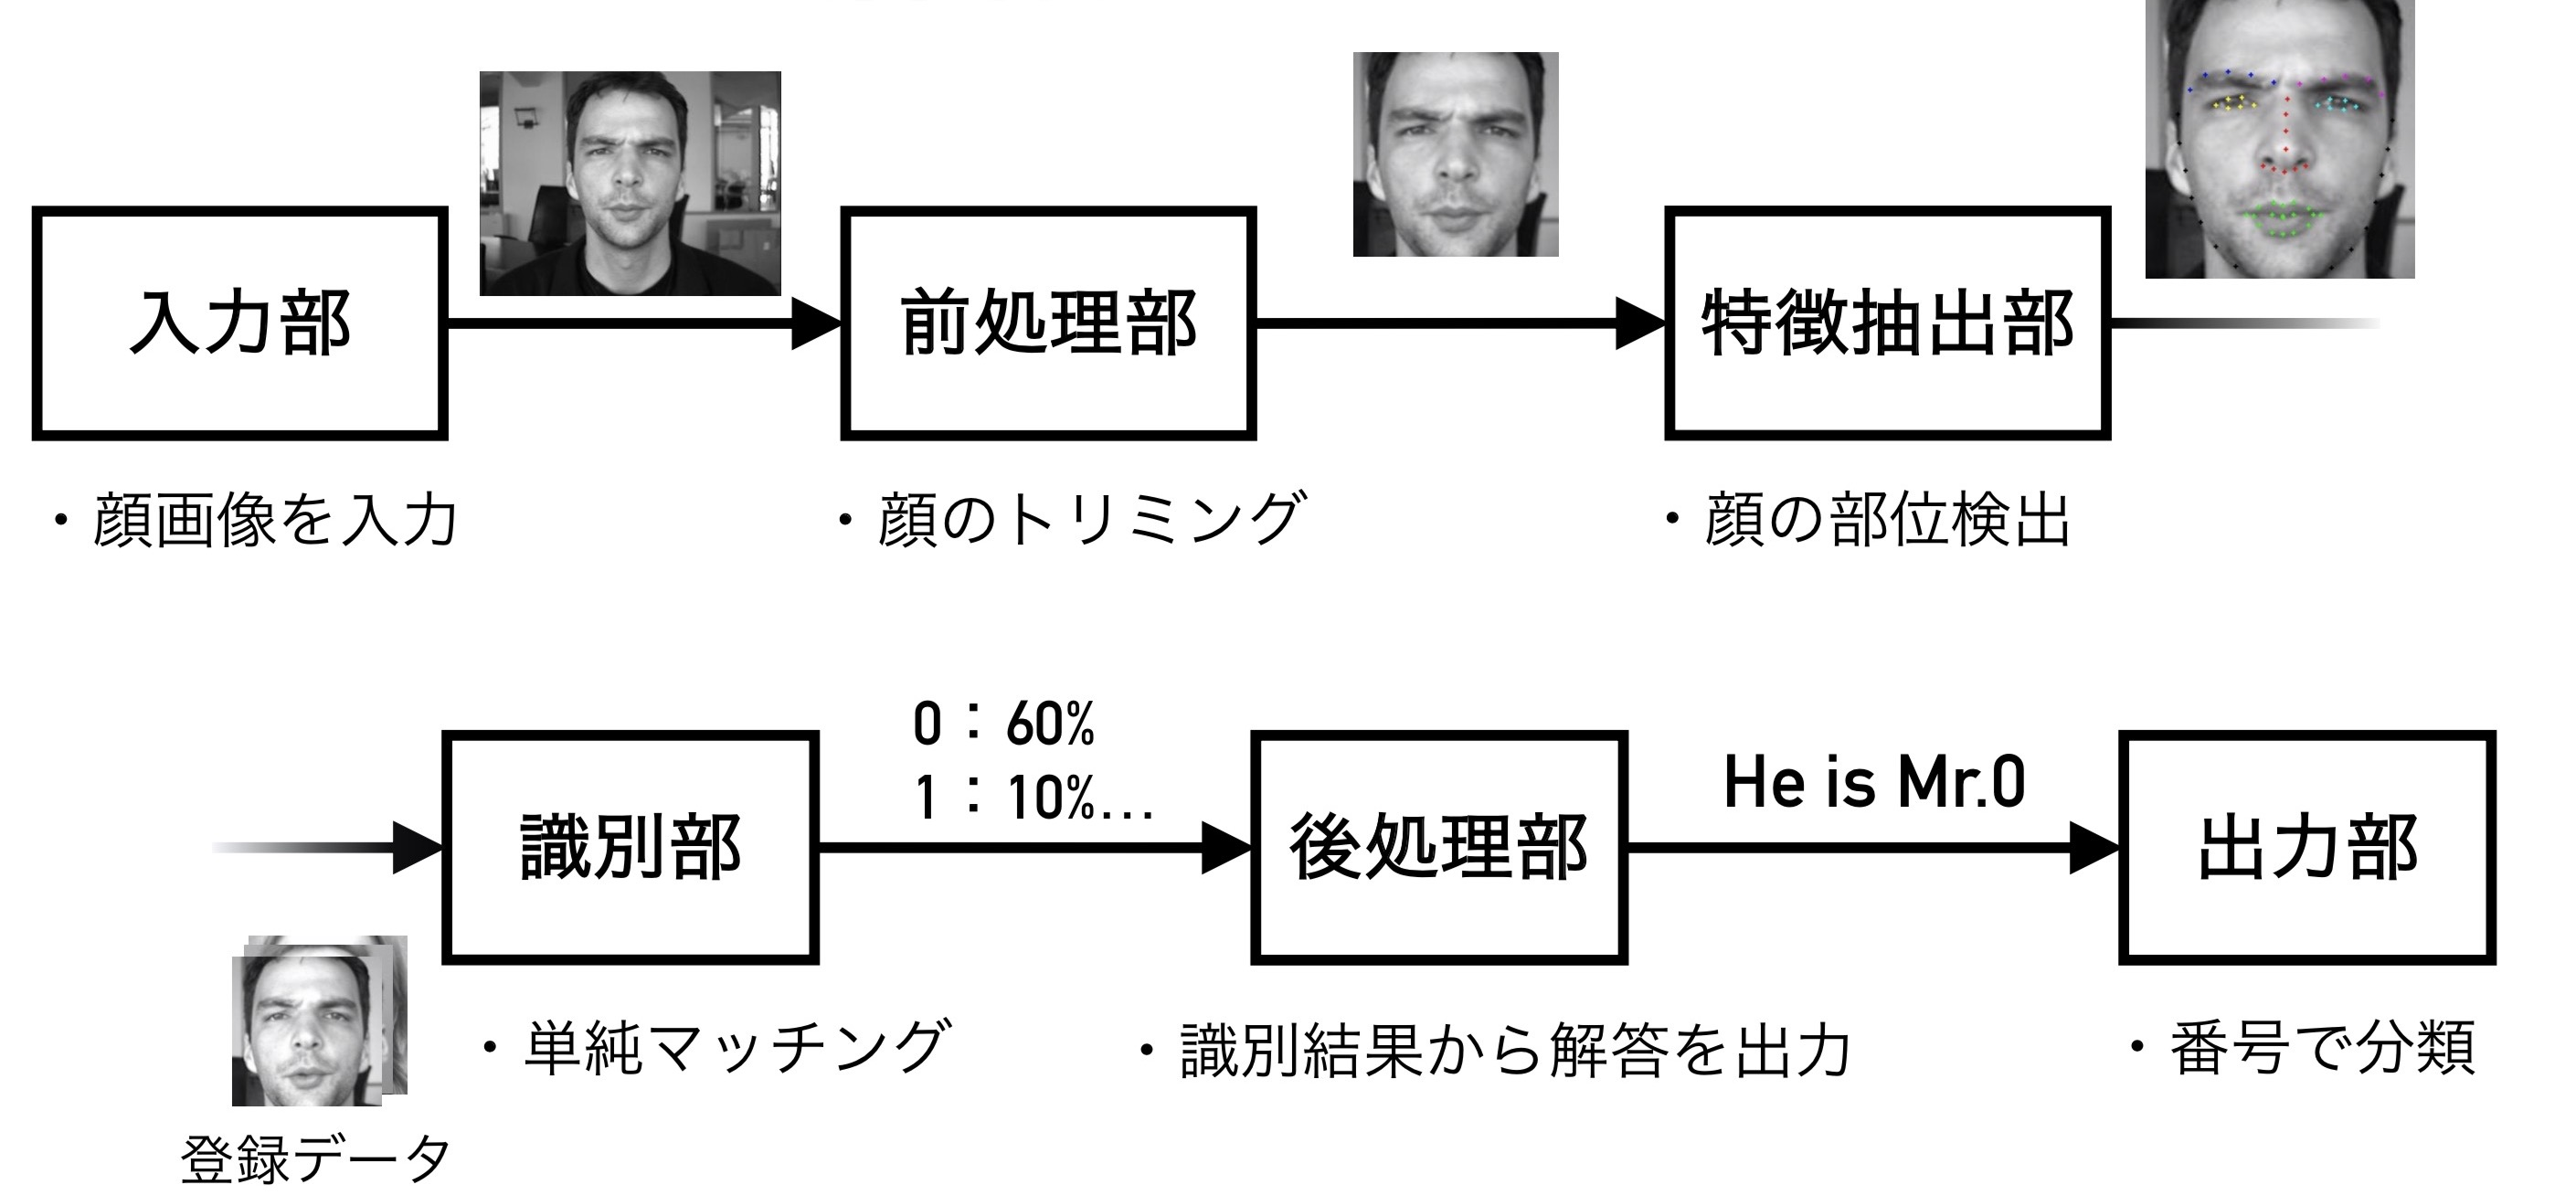
\includegraphics[width=10cm,clip]{images/system.jpg}
		\caption{システムの概要}
		\label{system}
	\end{figure}
	図\ref{system}の各手順について、採用した手法およびそれぞれの機能をどのように実装したか、及び該当プログラムについて説明する。なお、プログラムは付録として末尾に記載している。
	\subsection{入力部}
	入力部では、与えられた画像を読み込む。MATLABで作成したプログラムでは、使用する特徴量及び識別アルゴリズムを選択する処理も入力部で同時に行う。

	\begin{itemize}
		\item SAISYUU.m … パスを指定し、Pythonで顔検出および正規化された画像をMATLABに読み込む。
		\item preprocessingOpenCV.py … OpenCVを用いて画像の読み込みを行う。画像はフォルダのパスを指定し、フォルダ内のjpgファイルを読み込むように実装した。
	\end{itemize}
	\subsection{前処理部}
	\subsubsection{顔検出}
	与えられたデータセットの画像は人物のみでなく、背景も写ってしまっているため、識別する人物の顔だけを抽出する必要がある。

	\begin{itemize}
		\item preprocessingOpenCV.py … 画像を入力すると、顔を検出し、切り取った画像を出力する。
	\end{itemize}
	\subsubsection{正規化}
	顔を検出し、トリミングした場合、画像によって大きさに差異が生まれる。そこで、まず画像サイズの統一化を行なった。その後、画像の明るさによる誤識別を防止するため、画素値のヒストグラムを平坦化することで輝度を調整した。
	\begin{itemize}
		\item preprocessingOpenCV.py … 上記の顔検出を行なった後、輝度の調整を行う。
	\end{itemize}

	なお、後述する「\ref{feature} 特徴抽出部」中のDCT、HOGの特徴量を使用する場合にはCanny法と呼ばれるエッジ検出をおこなった。なお、Canny法はエッジ検出の一種で、ガウシアンフィルタを使って平滑化の処理をした後に微分をする。その微分画像の勾配からエッジを検出する方法である。

	\begin{itemize}
		\item SAISYUU.m … Canny法によるエッジ検出を行った。
		\item DCT.py … Canny法によるエッジ検出を行った。
	\end{itemize}
	\subsection{特徴抽出部}\label{feature}
	今回の実験では3つの特徴量を画像データから抽出した。
	\subsubsection{二次元離散コサイン変換(DCT)}
	画像を余弦波の周波数と係数成分へと変換する方法。画像のエネルギーは低域成分に集中しているため、変換後の周波数成分から低域の部分のみを特徴量として使用する。

	\begin{itemize}
		\item funcDCT.m … 画像を引数として渡す関数。DCT変換を行い、低周波成分を抜き出したものを特徴量として使用。
		\item DCT.py … 画像のDCT変換を行い、低周波成分を抽出する。
	\end{itemize}
	\subsubsection{HOG(Histograms of Oriented Gradients)}
	局所領域 (セル) の画素値の勾配方向ヒストグラムを特徴量としたもの。
	各ピクセルの輝度から勾配を求めた後、セル領域ごとにヒストグラムを求める。それをブロックごとに正規化し、特徴量を抽出する。今回の実験ではセルのサイズを8×8のもの(HOG8)と16×16のもの(HOG16)の二種類を使用した。

	\begin{itemize}
		\item funcHOG.m … 画像を引数として渡す関数。HOG特徴量を求めて特徴量として使用。
	\end{itemize}
	\subsubsection{Dilbを使った顔パーツの部位情報}
	Pythonのライブラリである、Dlibを使用して、顔の部位情報から、各パーツの相対位置や距離を利用し、特徴量とした。MATLABではPythonで書き出されたcsvファイルを読み込んで使用した。

	\begin{itemize}
		\item SAISYUU.m … 各識別アルゴリズム内で顔パーツの部位情報を使用する際にPythonで作成されたcsvファイルを読み込んで使用。
	\end{itemize}
	\subsection{識別部}
	今回の実験では、5つの識別アルゴリズムを用いて入力画像がどの人物なのか識別を行なった。
	\subsubsection{単純マッチング}
	特徴量や画像の画素値をピクセルごとに比較し、誤差が最も低いデータが属するクラス(今回は人物)を解答する方法。

	\begin{itemize}
		\item SAISYUU.m … 入力部で指定した、単純マッチングに使用する特徴量や画像をそれぞれ準備する。そして、クエリに対する特徴量を求め、単純マッチングの関数を呼び出し、回答を受け取る。
		\item matching.m … 画像の画素値や指定された特徴量を用いて、与えられたクエリと、200個のデータベースそれぞれに対しての距離計算をしている。そして、クエリと最も距離が近くなったデータベースの画像を選び、その画像はどのクラス(人物)だったのかを判別する。
		\item processes.py … MATLABと同様に特徴量の比較を行い、誤差が最小となるクラスに分類する。
	\end{itemize}
	\subsubsection{k最近傍法(kNN)}
	特徴量でデータをプロットし、クエリの特徴量と近い場所にあるk個のデータの中で多数決をしてどのクラスに属するか解答する方法。

	\begin{itemize}
		\item SAISYUU.m … 特徴量を用いてkNNモデルを作成し、作成したkNNモデルを使用して多数決の結果と、その内訳を出力し、多数決の結果を回答として使用。リジェクト機能を使用する場合は、多数決の内訳をチェックし、それが条件を満たさない場合はリジェクトする(リジェクトの条件の詳細については後述)。
		\item labeling.m … kNNモデルを作成するときに特徴量とラベルを引数として渡す必要があるため、その二つを作成するための関数。
		\item processes.py … 上記のMATLABとほぼ同じ仕様である。k近傍のk及び特徴量の比較に使う距離の指定はできるように実装した。
	\end{itemize}
	\subsubsection{部分空間法}
	特徴量を使ってベクトルを作成し、クエリの特徴量を用いて作成したベクトルと最も類似しているクラスを出力する方法。

	\begin{itemize}
		\item SAISYUU.m … データベースの特徴量から1人当たり10本のベクトルを作成し、その10本のベクトルの平均をとってその人物の代表ベクトルを決定する。これを20人分繰り返し、最後にその代表ベクトルとクエリの特徴量から作ったベクトルと、20人分の代表ベクトルを比較し、最も近似する代表ベクトルを持つ人物を回答する。リジェクト機能を使用する場合は、類似度(2つのベクトル間の角度)が閾値よりも大きいかどうか判定し、類似度が小さい(角度が大きい)場合はリジェクトを行う。
	\end{itemize}
	\subsubsection{畳み込みニューラルネットワーク(CNN)及びニューラルネットワーク(NN)}
	顔を切り出し、前処理を施した画像を入力としCNNを通し、どのクラスに属するかを出力する方法。ネットワークの構成は、畳み込み層-プーリング層-DropOut層-畳み込み層-プーリング層-DropOut層とした。活性化関数はReLU関数を使用した。DropOutの確率は0.5とし、プーリングのウィンドウサイズは2とした。ニューラルネットワークでは、特徴量を入力とし、中間層3層でそれぞれ1024ニューロンにした。出力は、0〜19のクラス値とした。

	\begin{itemize}
		\item processes.py … CNNとNNは、pytorchを用いて実装した。processesクラスのCNNクラス及び、eval\_net関数、train\_net関数が実際の処理の内容である。train\_netクラスではネットワークの訓練を行い、eval\_net関数では予測結果を算出する。予測された結果を使用し、精度をCNNクラスで計算し、それを返すという構成になっている。
	\end{itemize}

	\subsubsection{LightGBM}
	特徴量抽出部で抽出した特徴量を使用し、Gradient BoostingライブラリであるLightGBMを使用し、入力された特徴量はどのクラスに属するかを出力する方法。boostingの概略として、決定木の弱識別機を直列に複数並べ、これらを訓練し、最終的に弱識別器の予測値を線形結合した値を出力として得るというものである。

	\begin{itemize}
		\item preprocess.py … preprocessクラスのlightGBMクラスが実際の処理の内容である。評価指標としてmulti errorを使用し、学習率は0.1として、繰り返し数を200、early stoppingを100とした。これらの設定はparamsディクショナリにまとめてある。最終的に、受け取った特徴量を元に学習を行い、その後訓練データで一番精度が良かった繰り返し数のパラメータで予測を行い正解率を返すという構成になっている。
	\end{itemize}

	\subsection{出力部}
	今回の実験では正答率を求める必要があるため、出力した結果が正しいかどうかを判定するプログラムを追加した。
	\begin{itemize}
		\item SAISYUU.m … 正解ラベルを作成し、各手法によって回答された答えと正解ラベルを比較して正答率とリジェクト機能によってはじかれなかった個数を算出し、表示した。
		\item final\_gui.py … PyQtを用いて作成したGUI上でcsvファイルを読み込むことで精度を表示するように実装した。
	\end{itemize}
	\newpage
	\section{実験結果}
	各手法での正解率は表\ref{result}のようになった。
	\begin{table}[H]
		\begin{center}
			\caption{各識別手法と特徴量の組み合わせによる正解率[\%]}
			\label{result}
			\scalebox{0.7}[0.7]{
			\begin{tabular}{|c|c|c|c|c|c|c|c|}\hline
									& 単純マッチング	& K-NN(5)	& 部分空間法	& Neural Network	& LightGBM	& ピクセルマッチング			& CNN   \\ \hline \hline
				各部位の大きさと位置	& 53.44			& 48.28		& 43.10		& 50.00				& 39.66		& -							& -		\\ \hline
				CannyありDCT15		& 82.76			& 74.14		& 67.24		& 72.41				& 48.28		& \multirow{4}{*}{53.44}	& \multirow{4}{*}{65.52}		\\ \cline{1-6}
				CannyなしDCT15		& 51.72			& 44.83		& 50.00		& 56.90				& 50.00		&							&		\\ \cline{1-6}
				HOG8				& 72.41			& 68.97		& 41.38		& 62.07				& 43.1		&							&		\\ \cline{1-6}
				HOG16				& 75.86			& 75.86		& 62.07		& 70.69				& 48.28		&							&		\\ \hline
		    \end{tabular}
		    }
		\end{center}
	\end{table}

	\section{考察}
	\subsection{リジェクト機能}
	MATLABで実装された各認識アルゴリズムにおいて、正答率が高かった特徴量を用いたものに対して「データベースに登録されていない人物をはじく機能(リジェクト機能)」を実装した。リジェクトの方法は「距離や角度に対して閾値を用いてその閾値を上回った場合リジェクトする」方法(単純マッチング、部分空間法)と「距離が近かった5つが同一でない場合にリジェクトする」方法をとった。その時の精度を表4に、再現率を表5に示す。なお、ここでの精度とは「識別器がリジェクトしなかったものに対して正しく分類できた割合」、再現率とは「データベースに登録されているクエリ(56枚)に対して正しく分類した割合」とする。また、今回の実験ではシステムが「顔認証」であるため、精度ができるだけ100\%に近づけるようにし、その条件の下で最大となる再現率を表5に示した。

	\begin{table}[H]
		\begin{center}
			\caption{リジェクト機能を使用した際の適合率と再現率[\%]}
			\label{recall_precision}
			\begin{tabular}{|c|c|c|c|}\hline
									& 単純マッチング	& K-NN(5)	& 部分空間法 \\ \hline \hline
				CannyありDCT15 適合率	& 100			& 87.88		& 100		\\ \hline
				CannyありDCT15 再現率	& 46.43			& 57.14		& 25.00		\\ \hline
				HOG16 適合率			& 100			& 96.43		& 100		\\ \hline
				HOG16 再現率			& 48.21			& 50.00		& 37.93		\\ \hline
		    \end{tabular}
		\end{center}
	\end{table}
	表\ref{result}と表\ref{recall_precision}を比較すると、リジェクト機能を搭載することによって精度は向上しているが、その代わり再現率が下がるというトレードオフの関係が成り立っていることがわかる。また、表\ref{result}の結果では単純マッチングおよび部分空間法ではDCTのほうが正答率が高く、良い特徴量であると考えられていた。しかし、表4、表5をみるとその2つの識別アルゴリズムではともに適合率は100\%であっても、HOGのほうが再現率は高くなっているため、リジェクト機能を使用する際にはHOG特徴量のほうが有用であると考えられる。また、k最近傍法では、精度を100\%にすることができなかったため、リジェクト機能を搭載する場合に用いる識別アルゴリズムは単純マッチングか部分空間法が適しているのではないかと考える。

	\newpage
	\section{付録}
	\subsection{MATLABファイル}
\begin{lstlisting}[caption=SAISYUU.m,label=saisyuu]
	clc
	clear
	%% DBの実装
	c = 20; % クラス総数
	n = 10; % 1クラス当たりの学習パターン数

	% データベースの読み込み
	path = 'M:\project\dataset2\DB\jpeg\';
	for i=1:c
	  for j=1:n
	    str = strcat(path, num2str(n*(i-1)+j-1, '%03d'), '.jpg');
	    img = imread(str);
	    img = edge(img, 'Canny',[],2);
	    DB(:,:,n*(i-1)+j) = img;
	  end
	end

	% クエリの読み込み
	Qpath  = 'M:\project\dataset2\Query\jpeg\';
	D = dir('M:\project\dataset2\Query\jpeg\*.jpg');
	for i=1:length(D)
	  name = strcat(Qpath, D(i).name);
	  img = imread(name);
	  img = edge(img, 'Canny', [], 2);
	  Query(:,:,i) = img;
	end
	%% 使用する機能選択
	fprintf('どのアルゴリズムを使用しますか?\n')
	prompt = '0=単純マッチング(輝度値),1=単純マッチング(DCT),2=単純マッチング(HOG),3=単純マッチング(Face_Parts),4=KNN(DCT),5=KNN(HOG),6=KNN(Face_Parts),7=部分空間(DCT),8=部分空間(HOG),9=部分空間(Face_Parts)\n';
	hanbetu = input(prompt);
	fprintf('リジェクト機能を使用しますか?\n')
	prompt = '1=Yes,0=No\n';
	RJ = input(prompt);
	answer = zeros(1, 58);
	%% 単純マッチング
	if (hanbetu >= 0 && hanbetu <= 3)
	  %特徴量のDB作成
	  if (hanbetu >= 1 && hanbetu <= 2)
	    for i=1:200
	        img=DB(:,:,i);
	      if hanbetu == 1
	        m_feature = funcDCT(img);
	      else
	        m_feature = funcHOG(img);
	      end
	      m_DB(i,:) = m_feature;
	    end
	  end
	  if hanbetu == 3
	    m_DB = csvread('M:\project\dataset4\DB\csv\FP.csv');
	    Query_feature = csvread('M:\project\dataset4\Query\csv\QFP.csv');
	  end
	  %単純マッチングによる回答
	  for i=1:length(D)
	    if hanbetu == 0
	      Q_feature = double(Query(:,:,i));
	    elseif hanbetu == 1
	      Q_feature = funcDCT(Query(:,:,i)) ;
	    elseif hanbetu == 2
	      Q_feature = funcHOG(Query(:,:,i)) ;
	    elseif hanbetu == 3
	      Q_feature = Query_feature(i,:) ;
	    end
	    if hanbetu == 0
	      answer(i) = matching(DB, Q_feature, hanbetu, RJ);
	    else
	      answer(i) = matching(m_DB, Q_feature, hanbetu, RJ);
	    end
	  end
	end
	%% KNN
	if(hanbetu >= 4 && hanbetu <=6)

	  %knnモデルの作成
	  [fDB, C] = labeling(DB, hanbetu); %特徴量のラベリング
	  model = fitcknn(fDB, C);
	  model.NumNeighbors = 5;

	  %knnモデルによる回答
	  if hanbetu == 6
	    Query_filename = 'M:\project\dataset4\Query\csv\QFP.csv';
	    Query_feature = csvread(Query_filename);
	  end
	  for i=1:length(D)
	    testImg = Query(:,:,i); %クエリの取得
	    if hanbetu == 4
	      dctF = funcDCT(testImg);
	      [answer(i), score(i,:)] = predict(model, dctF);
	    elseif hanbetu == 5
	      hogF = funcHOG(testImg);
	      [answer(i), score(i,:)] = predict(model, hogF);
	    elseif hanbetu == 6
	      faceF = Query_feature(i,:);
	      [answer(i), score(i,:)] = predict(model, faceF);
	    end
	  end
	  %リジェクト領域
	  if RJ == 1
	    score2 = score.';
	    [MA,I] = max(score2);
	    for i=1:58
	      if MA(i) > 0.9
	        answer(i) = I(i) - 1;
	      else
	        answer(i) = 999;
	      end
	   	 end
	  end
	end
	%% 部分空間(DCTを特徴量とする場合)
	if(hanbetu >= 7 && hanbetu <=8)
	  if hanbetu == 7
	    feature_num = 225;
	  else
	    feature_num = 2916;
	  end
	  %DB部分
	  for i=1:200
	    img = DB(:,:,i);
	    if hanbetu == 7
	      db_feature_list(i,:) = funcDCT(img);
	    else
	      db_feature_list(i,:) = funcHOG(img);
	    end
	  end

	  %クエリ部分
	  for i=1:58
	    img = Query(:,:,i);
	    if hanbetu == 7
	      Query_feature(i,:) = funcDCT(img);
	    else
	      Query_feature(i,:) = funcHOG(img);
	    end
	  end
	  for i=1:58
	    Query_feature(i, feature_num+1) = sqrt(sumsqr(Query_feature(i,:)));
	  end
	end
	%% 部分空間(顔のパーツを特徴量として扱う場合)
	if hanbetu == 9
	  %DB部分
	  DB_filename = 'M:\project\dataset4\DB\csv\FP.csv';
	  db_feature_list = csvread(DB_filename);
	  feature_num = 20;

	  %クエリ部分%
	  Query_filename = 'M:\project\dataset4\Query\csv\QFP.csv';
	  Query_feature = csvread(Query_filename);
	  %クエリのサイズ計算
	  for i=1:58
	    Query_feature(i, feature_num+1) = sqrt(sumsqr(Query_feature(i,:)));
	  end
	end
	%% 部分空間回答部
	if(hanbetu >= 7 && hanbetu <= 9)
	  %平均値計算
	  sub_space = zeros(20, feature_num+1);
	  test = zeros(200, feature_num);
	  for i=1:20 %i=人数
	  	for j=1:10 % i人目について10枚ずつ処理
	      for k=1:feature_num %特徴量が20個
	        test(j,k) = db_feature_list((i-1)*10+j, k);
	      end
	    end
	    %平均値をとる
	    M = mean(test);
	    for k=1:feature_num
	      sub_space(i,k) = M(k);
	    end
	    zettai = sqrt(sumsqr(sub_space(i,:)));
	    sub_space(i, feature_num+1) = zettai;
	  end

	  %部分空間法による回答
	  hairetu = zeros(58,20);
	  for j=1:58
	    for i=1:20
	      for k=1:feature_num
	        hairetu(j,i) = hairetu(j,i) + Query_feature(j,k) * sub_space(i,k);
	      end
	      hairetu(j,i) = acos(hairetu(j,i) / (Query_feature(j,feature_num+1) * sub_space(i,feature_num+1)) );
	    end
	  end
	  [S, answer] = min(hairetu, [], 2);

	  %リジェクト領域
	  for i=1:58
	    if hanbetu == 8
	      sikiiti = 0.95;
	    elseif hanbetu == 7
	      sikiiti = 0.47;
	    end
	    if(RJ == 1 && S(i) > sikiiti)
	      answer(i) = 999;
	    else
	      answer(i) = answer(i) - 1;
	    end
	  end
	end
	%% Answer check

	% Qラベルの作成
	A = zeros(1, 8);
	Qlabels = A;
	nums = [3, 3, 4, 3, 3, 4, 2, 3, 3, 3, 3, 3, 3, 2, 1, 1, 1, 1, 2, 2];
	for i=1:20
	  A = ones(1, nums(i) ) * i;
	  Qlabels = horzcat(Qlabels, A);
	end

	% 正解率の判定
	correctNum = 0;
	PassNum = 0;
	for i=1:length(D)
	  if(answer(i) > 19 && RJ == 1)
	      PassNum = PassNum + 1;
	  end
	  if(answer(i) == Qlabels(i))
	      correctNum = correctNum + 1;
	  end
	end

	sprintf('正解率: %.4f', correctNum / ( length(D) ) )
	sprintf('精度 %.4f',correctNum / ( PassNum ))
\end{lstlisting}

\begin{lstlisting}[caption=matching.m,label=matching]
	function number = matching(DB, Query, hanbetu, RJ)
	  %単純マッチング関数(関数Mファイル)
	  %クエリ画像XとDBの画像をピクセル毎に比較し、二乗誤差が最も小さい人物を出力する
	  for i=1:200
	    if hanbetu == 0
	      A = double(DB(:,:,i));
	    elseif (hanbetu >= 1 && hanbetu <= 3)
	      A = DB(i,:);
	    end
	    D = (Query - A).^2;
	    distance(i) = sum(sum(D));
	  end

	  [minimum, index] = min(distance);
	  %リジェクト領域
	  if RJ == 1
	      if hanbetu == 1
	          sikiiti = 140;
	      elseif hanbetu == 2
	          sikiiti = 57;
	      end
	    if minimum > sikiiti
	      index = 10000;
	    end
	  end

	  number = ceil(index / 10) - 1;
	end
\end{lstlisting}

\begin{lstlisting}[caption=funcDCT.m,label=funcDCT]
	function dctFeature = funcDCT(img)
	  % DCT特徴量
	  img4 = dct2(double(img)); %2次元DCT
	  imgdctlow = img4(1:15, 1:15); %低周波成分の抜き出し
	  dctFeature = reshape(imgdctlow, [1, 15*15]); %1次元化
	end
\end{lstlisting}

\begin{lstlisting}[caption=funcHOG.m,label=funcHOG]
	function hogFeature = funcHOG(img)
	  % DCT特徴量
	  hogFeature = extractHOGFeatures(img, 'CellSize', [16 16]);
	end
\end{lstlisting}

\begin{lstlisting}[caption=labeling.m,label=labeling]
	function [fDB,C] = labeling(DB,hanbetu)
	  %特徴量のDB作成関数

	  if hanbetu == 6
	    DB_filename = 'M:\project\dataset4\DB\csv\FP.csv';
	    feature_list = csvread(DB_filename);
	  end

	  for i=1:200
	    %DBのi枚目を読み込む
	    img = DB(:,:,i);

	    %i枚目の特徴量計算
	    if hanbetu == 4
	      feature = funcDCT(img); %dctの場合
	    elseif hanbetu == 5
	      feature = funcHOG(img);
	    elseif hanbetu == 6
	      feature = feature_list(i,:);
	    end

	    %特徴量のDB
	    fDB(:,i) = feature;
	    %正解ラベル
	    C(i) = fix( (i-1) / 10);
	  end

	  C = transpose(C);
	  fDB = transpose(fDB);
	end
\end{lstlisting}

	\newpage
	\subsection{Pythonファイル}
	\lstinputlisting[caption=processes.py,label=processes]{processes.py}
	\lstinputlisting[caption=preprocessingOpenCV.py,label=preprocessingOpenCV]{preprocessingOpenCV.py}
	\lstinputlisting[caption=preprocessingDlib.py,label=preprocessingDlib]{preprocessingDlib.py}
	\lstinputlisting[caption=DCT.py,label=DCT]{DCT.py}
	\lstinputlisting[caption=final\_gui.py,label=final_gui]{final_gui.py}
\end{document}